\documentclass[a4paper, 11pt]{book}
\usepackage{/home/nora/Documents/Enseignement/Prepa/bpep/fichiers_utiles/preambule}

\makeatletter
\renewcommand{\@chapapp}{Kh\^olles MPSI -- semaine}
\makeatother
\renewcommand\thechapter{16}

\toggletrue{corrige}  % décommenter pour passer en mode corrigé

 % IMPORTS automatiques
\newcommand{\f}[2]{{
		\mathchoice
		{\dfrac{#1}{#2}}
		{\dfrac{#1}{#2}}
		{\frac{#1}{#2}}
		{\frac{#1}{#2}}
}}

\newcommand{\e}[1]{{}_{\text{#1}}}

 % fin des IMPORTS automatiques

\begin{document}

\chapter{Sujet 1\siCorrige{\!\!-- corrig\'e}}
\resetQ
\section{Anneau sur une tige en rotation}

\noindent
\enonce{%
	\begin{minipage}{0.70\linewidth}
		On considère un petit anneau M de masse $m$ considéré comme ponctuel, soumis
		à la pesanteur et susceptible de se déplacer sans frottement le long d'une
		tige OA horizontale dans le plan ($x$O$y$), de longueur $\ell$, effectuant
		des mouvements de rotation caractérisés par une vitesse angulaire $\w$
		constante autour d'un axe fixe vertical $\D$ passant par son extrémité O. Le
		référentiel lié au laboratoire est considéré comme galiléen. On considère~:
		\bigbreak
		\begin{itemize}
			\item le repère cartésien $(\Or,\ex,\ey,\ez)$ fixe dans le référentiel
			      du laboratoire et associé aux axes $x$, $y$ et $z$~;
			\item la base cylindrique locale $(\er,\et,\ez)$ associée au point M.
		\end{itemize}
		\bigbreak
	\end{minipage}
	\hfill
	\begin{minipage}{0.25\linewidth}
		\begin{center}
			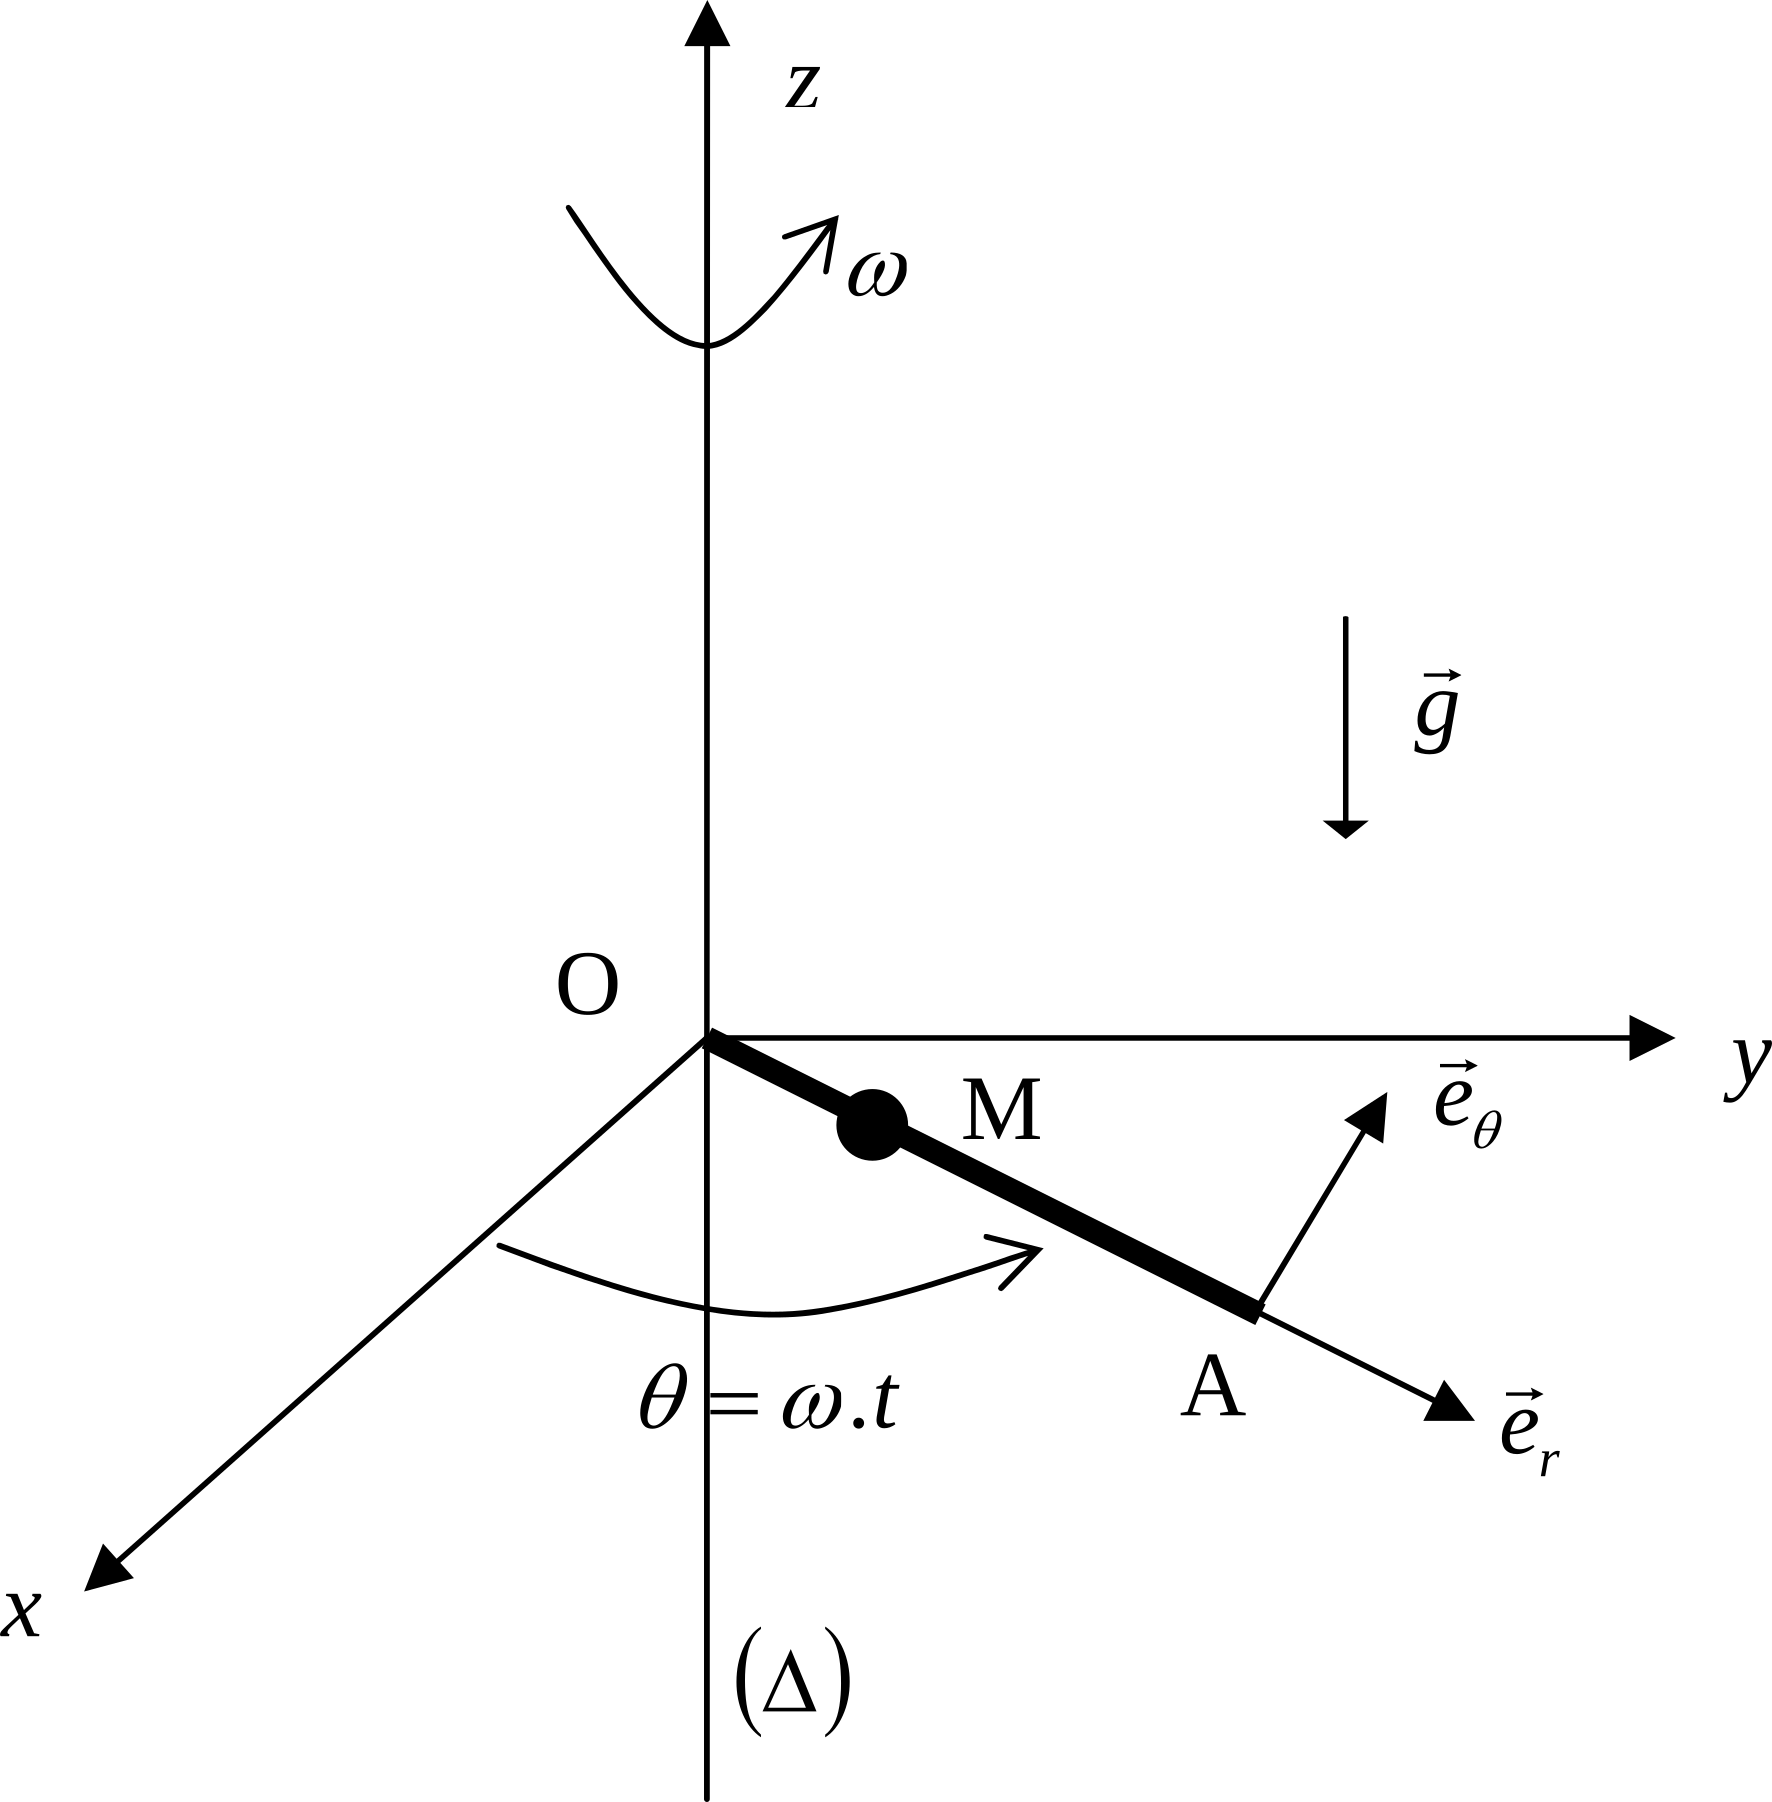
\includegraphics[width=\linewidth]{../figures/anneau_tige_rot-plain}
		\end{center}
	\end{minipage}
	L'anneau est libéré sans vitesse initiale par rapport à la tige, à une
	distance $r_0$ du point O (avec $r_0 < \ell$). On repère la position de
	l'anneau sur la tige par la distance $r = \OMr$ entre le point O et l'anneau
	M.
}
\QR{%
	Faire un bilan des forces agissant sur l'anneau en les projetant dans
	la base $(\er,\et,\ez)$. En appliquant le
	principe fondamental de la dynamique, établir l'équation différentielle
	vérifiée par $r(t)$.
}{%
	\begin{minipage}[t]{0.60\linewidth}
		\begin{itemize}[label=$\diamond$, leftmargin=10pt]
			\bitem{Système~:} \{anneau\} point matériel M de masse $m$
			\bitem{Référentiel~:} terrestre supposé galiléen
			\bitem{Repère~:} cylindrique $(\Or,\er,\et,\ez)$
			\bitem{Repérage~:}
			\begin{align*}
				\OM & = r\er                                        \\
				\vf & = \rp\er + r\tp\et                            \\
				    & = \rp\er + r\w\et                             \\
				\af & = \rpp\er + \rp\tp\et + \rp\w\et - r\w^2\er +
				\underbracket[0.4pt]{\of}_{\dot{\w}=0}              \\
				    & = (\rpp -r\w^2)\er +2r\w\et
			\end{align*}
		\end{itemize}
	\end{minipage}
	\hfill
	\begin{minipage}[t]{0.35\linewidth}
		~
		%\vspace*{6cm}
		\begin{center}
			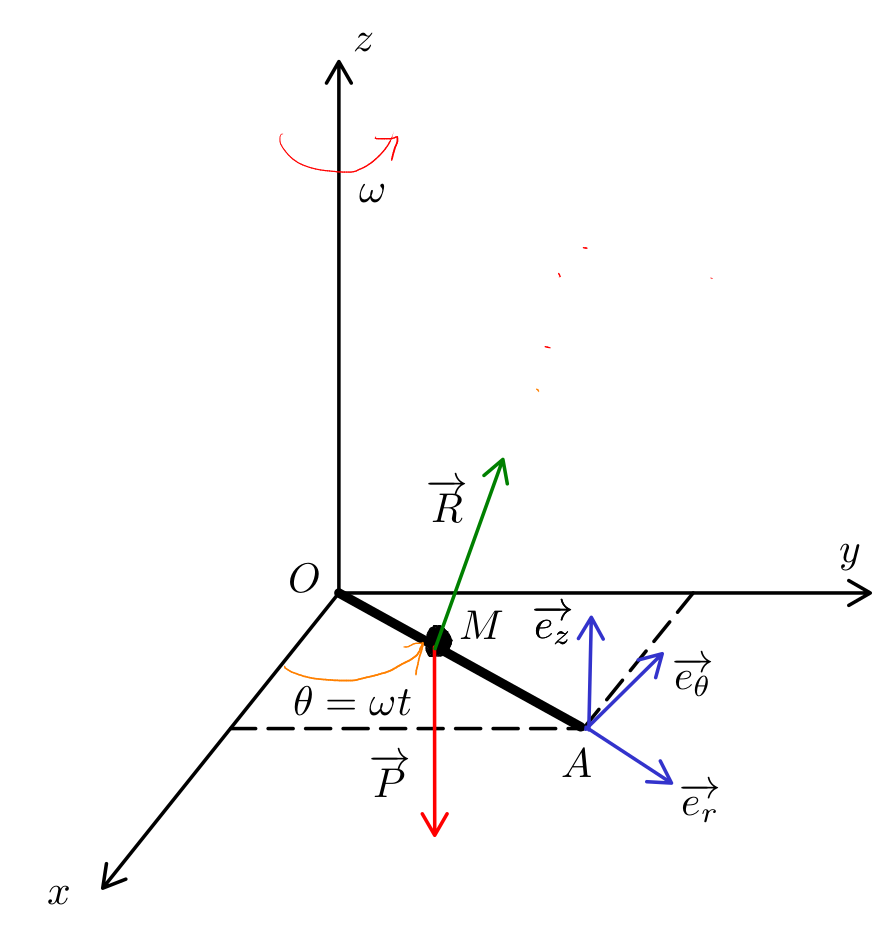
\includegraphics[scale=.18]{../figures/tige_rot_corr}
		\end{center}
	\end{minipage}
	\begin{itemize}[label=$\diamond$, leftmargin=10pt]
		\bitem{Conditions initiales~:}
		\[
			r(0) = r_0
			\qet
			\vf(0) = \of \Ra \rp(0) = 0
		\]
		\bitem{BDF~:} pas de frottements donc pas de composante sur $\er$~:
		\[
			\begin{array}{ll}
				\textbf{Poids}            & \Pf = m\gf = -mg\ez     \\
				\textbf{Réaction support} & \Rf = R_\tt\et + R_z\ez
			\end{array}
		\]
		\bitem{PFD~:}
		\begin{gather*}
			m\af = \Pf + \Rf
			\Lra
			\left\{
			\begin{aligned}
				m(\rpp-r\w^2) & = 0         \\
				2m\rp\w       & = R_\tt     \\
				0             & = -mg + R_z
			\end{aligned}
			\right.
		\end{gather*}
		\begin{empheq}[box=\fbox, left=\Lra\empheqlbrace]{align}
			\label{eq:tigerota}
			\Aboxed{
				\rpp - \w r &= 0
			}\\
			\label{eq:tigerotb}
			R_\tt &= 2m\rp\w\\
			\label{eq:tigerotc}
			R_z &= mg
		\end{empheq}
	\end{itemize}
}
\QR{%
	Intégrer cette équation différentielle en prenant en compte les
	conditions initiales définies précédemment, et déterminer la solution
	$r(t)$ en fonction de $r_0$, $\w$ et $t$.
}{%
	On résout~\eqref{eq:tigerota} avec l'équation caractéristique~:
	\begin{align*}
		\rpp -\w^2r & = 0
		\\\Ra
		s^2 - \w^2  & = 0
		\\\Lra
		s^2         & = \w^2
		\\\Lra
		\Aboxed{s   & = \pm\w}
	\end{align*}
	On a donc des solutions de la forme
	\begin{gather*}
		r(t) = A\exr^{\wt} + B\exr^{-\wt}
		\shortintertext{Or, avec les CI~:}
		\begin{aligned}
			r(0)        & = r_0
			\\\Lra
			\Aboxed{r_0 & = A+B}
		\end{aligned}
		\shortintertext{et}
		\begin{aligned}
			\rp(0)    & = 0
			\\\Lra
			0         & = A\w -B\w
			\\\Lra
			\Aboxed{A & = B}
		\end{aligned}
		\shortintertext{Soit}
		\\
		\boxed{A = B = \frac{r_0}{2}}
		\Ra
		\boxed{r(t) = \frac{r_0}{2}(\exr^{\wt} + \exr^{-\wt}) =
			r_0\cosh(\wt)}
	\end{gather*}
}
\QR{%
	Exprimer les composantes de la réaction $\Rf$ de la tige sur M dans la
	base $(\er,\et,\ez)$ en fonction de $m$, $g$, $\rp$ et $\w$.
}{%
	On reprend~\eqref{eq:tigerotb} et~\eqref{eq:tigerotc} avec $\rp =
		\w r_0\sinh(\wt)$~:
	\[
		\boxed{
			\Rf = 2mr_0\w^2\sinh(\wt)\et + mg\ez
		}
	\]
}
\QR{%
	Déduire de la question 2 le temps $\tau$ que va mettre l'anneau pour
	quitter la tige. On exprimera $\tau$ en fonction de $r_0$, $\ell$ et
	$\w$.
}{%
	L'anneau quitte la tige en $\tau$ quand $r(\tau) = \ell$, soit
	\begin{gather*}
		\ell = r_0\cosh(\wt)
		\\\Lra
		\boxed{\tau = \frac{1}{\w}\acosh(\wt)}
	\end{gather*}
}

\chapter{Sujet 2\siCorrige{\!\!-- corrig\'e}}
\resetQ
\section{Pendule conique}
\enonce{%
	\noindent
	\begin{minipage}{0.70\linewidth}
		Dans un champ uniforme de pesanteur $\gf$ vertical et vers le bas, un point
		matériel M de masse $m$ tourne à la vitesse angulaire $\w$ constante autour
		de l'axe (O$z$) dirigé vers le haut en décrivant un cercle de centre O et de
		rayon $R$. M est suspendu à un fil inextensible de longueur $L$ et de masse
		négligeable, fixé en un point A de (O$z$). L'angle $\a$ de (O$z$) avec AM
		est constant.
		\QR{%
			Quel système de coordonnées utiliser~?
		}{%
			On utilisera un repère cylindrique pour étudier la rotation.
		}
	\end{minipage}
	\hfill
	\begin{minipage}{0.25\linewidth}
		\begin{center}
			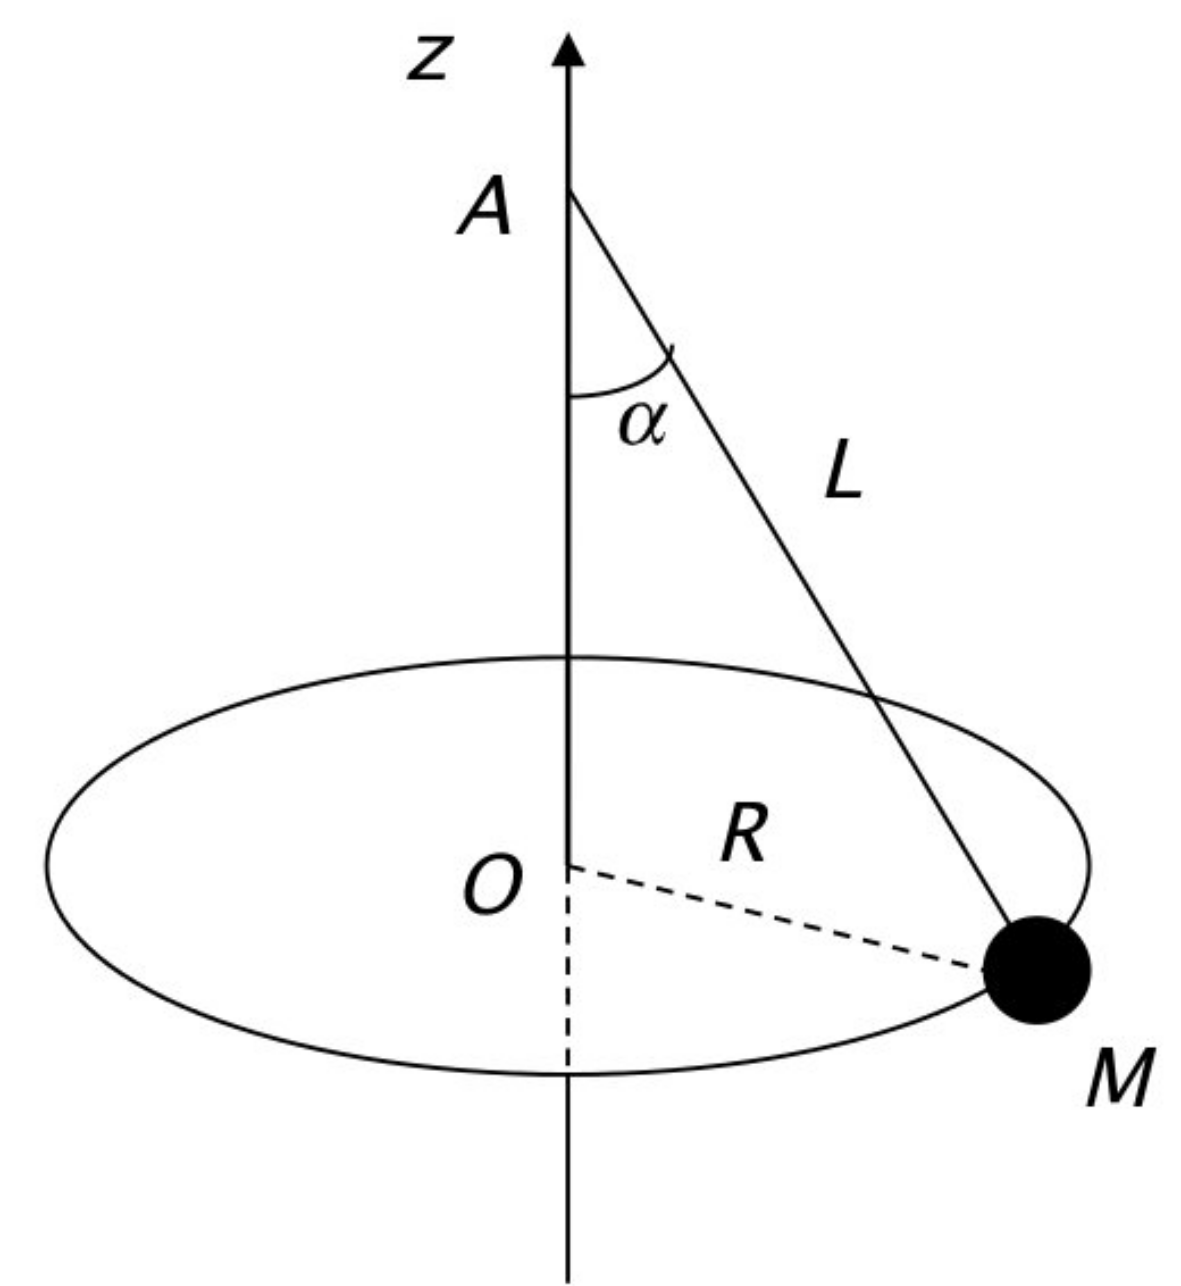
\includegraphics[width=\linewidth]{../figures/pendule_conique-plain}
		\end{center}
	\end{minipage}
}
\QR{%
	Effectuer un bilan des forces s'appliquant à la masse et les écrire
	dans la base choisie.
}{%
	\begin{itemize}[label=$\diamond$, leftmargin=10pt]
		\bitem{Système~:} \{M\} masse $m$
		\bitem{Référentiel~:} $\Rc\ind{labo}$ supposé galiléen
		\bitem{Repère~:} $(\Or, \ur, \ut, \uz)$ (voir schéma)
	\end{itemize} \smallbreak
	\begin{minipage}{0.65\linewidth}
		\begin{itemize}[label=$\diamond$, leftmargin=10pt]
			\bitem{Repérage~:} $R = \cte\Ra\dot{R} = 0$, $\tp = \w =
				\cte\Ra\dot{\w} = 0$~:
			\begin{align*}
				\OM       & = R\ur = L\sin\a\ur \\
				\vf_{\Mr} & = L\tp\sin\a\ut     \\
				          & = L\w\sin\a\ut      \\
				\af_{\Mr} & = -L\w^2\sin\a\ur
			\end{align*}
			\bitem{BDF~:}
			\[
				\begin{array}{ll}
					\textbf{Poids}   & \Pf = m\gf = -mg\uz             \\
					\textbf{Tension} & \Tf = T(-\sin\a\ur + \cos\a\uz)
				\end{array}
			\]
		\end{itemize}
	\end{minipage}
	\hfill
	\begin{minipage}{0.30\linewidth}
		\begin{center}
			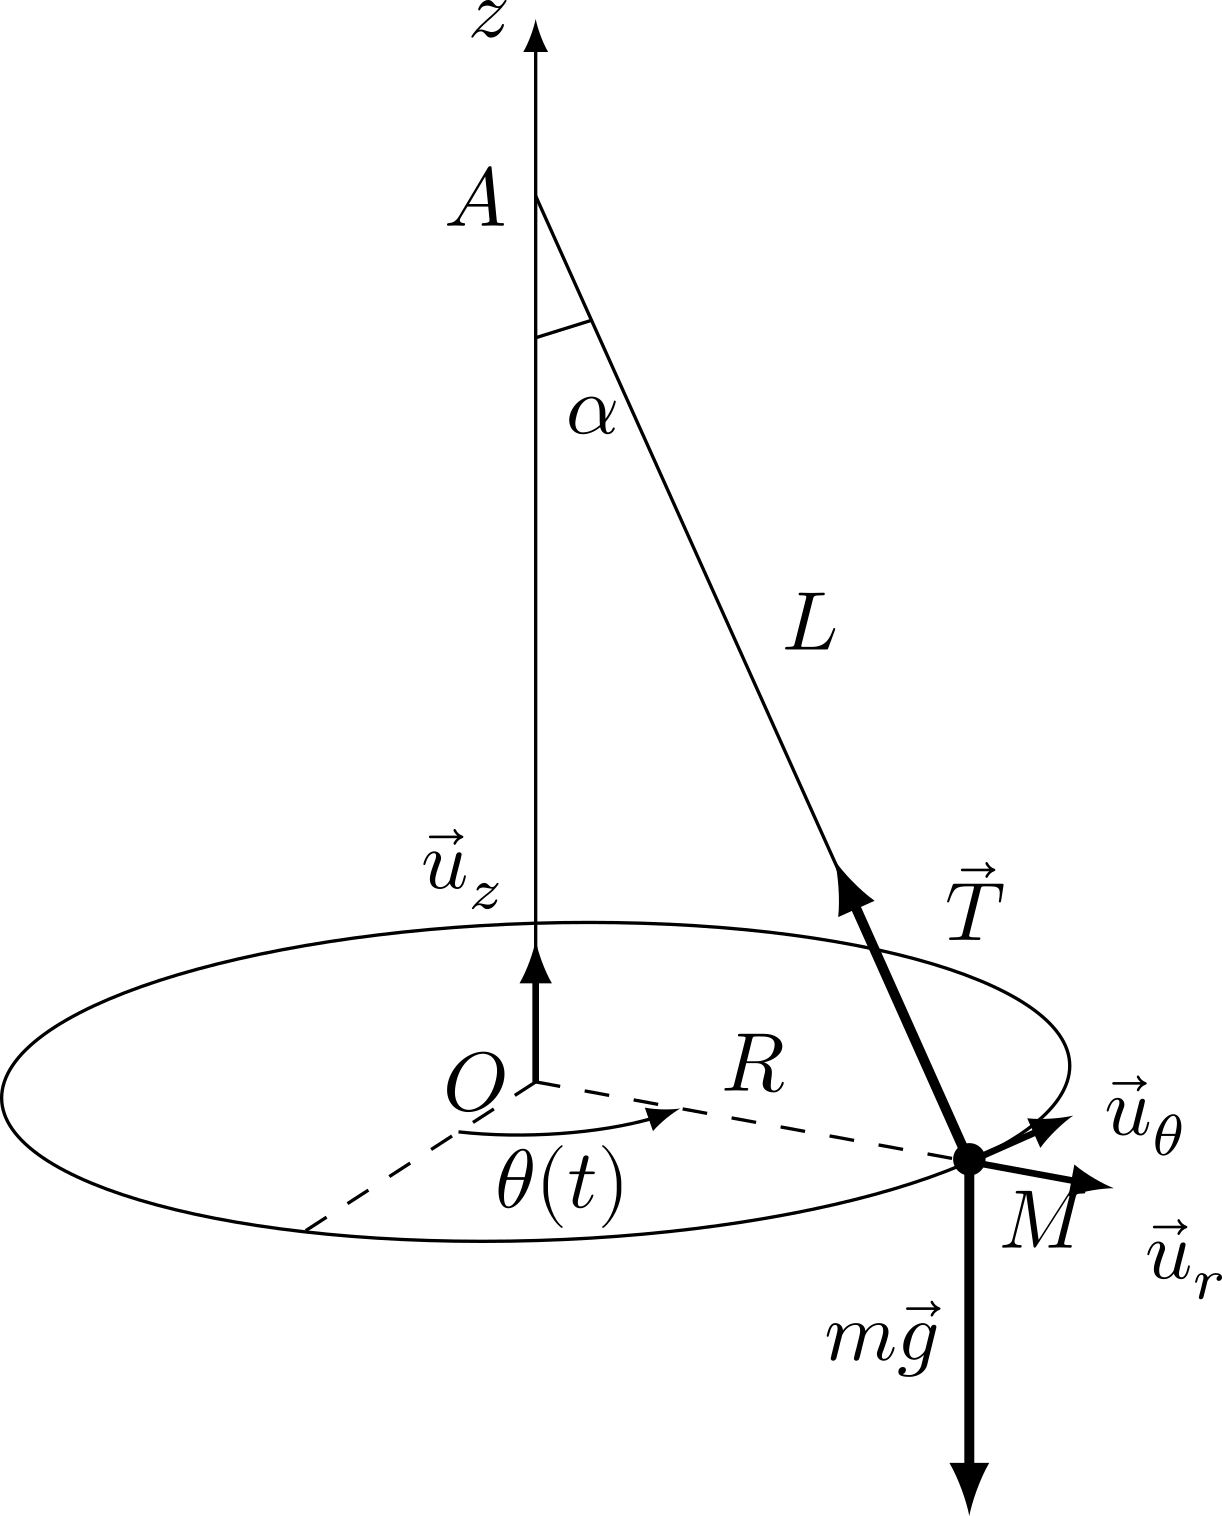
\includegraphics[width=\linewidth]{../figures/pendule_corr}
		\end{center}
	\end{minipage}
}
\QR{%
	Appliquer le PFD puis exprimer $\cos\a$ en fonction de $g$, $L$ et
	$\w$. En déduire que la vitesse angulaire doit forcément être supérieure
	à une vitesse angulaire limite $\w_{\lim}$ pour qu'un tel mouvement
	puisse être possible.
}{%
	On applique le PFD~:
	\begin{gather*}
		m\af = \Pf + \Tf
		\Lra
		\left\{
		\begin{aligned}
			-mL\w^2\cancel{\sin\a} & = -T\cancel{\sin\a} \\
			0                      & = T\cos\a -mg
		\end{aligned}
		\right.
		\Lra
		\left\{
		\begin{aligned}
			T & = mL\w^2            \\
			T & = \frac{mg}{\cos\a}
		\end{aligned}
		\right.
		\shortintertext{Soit}
		mL\w^2 = \frac{mg}{\cos\a}
		\Lra
		\boxed{\cos\a = \frac{g}{L\w^2}}
	\end{gather*}
	Pour que ce mouvement soit possible, il faut que $\cos\a < 1$, soit
	\begin{gather*}
		\frac{g}{L\w^2} < 1
		\Lra
		\boxed{\w \geq \sqrt{\frac{g}{L}} = \w_{\lim}}
	\end{gather*}
}
\QR{%
	Que dire du cas où $\w$ devient très grande~?
}{%
	Si $\w \gg \w_{\lim}$, alors $\cos\a \xrightarrow[\w \gg \w_{\lim}]{} 0$
	donc \fbox{$\a\xrightarrow[\w \gg \w_{\lim}]{} \pi/2$}~: le mouvement
	devient simplement circulaire, et se fait dans le plan horizontal
	contenant A.
}
\QR{%
	Application numérique~: calculer $\a$ pour $L = \SI{20}{cm}$ et $\w =
		\SI{3}{tours.s^{-1}}$.
}{%
	\leftcenters{On trouve}{\fbox{$\cos\a = \num{0.138} \Lra \a =
				\ang{82}$}}
}

\chapter{Sujet 3\siCorrige{\!\!-- corrig\'e}}
\resetQ
\subimport{/home/nora/Documents/Enseignement/Prepa/bpep/exercices/TD/ski/}{sujet.tex}

\end{document}
